\chapter{Architectural Design} \label{ch:architectural_design}


\section{Overview}
 At the high level, the system employs a client-server architecture. The client part consists of the web application running in a browser on a user's machine, whereas the server part is composed of web, DREAM, mail, and SQL servers. The high-level architecture is presented in the figure \ref{fig:high-level-architecture}.

\begin{figure}[H]
    \centering
    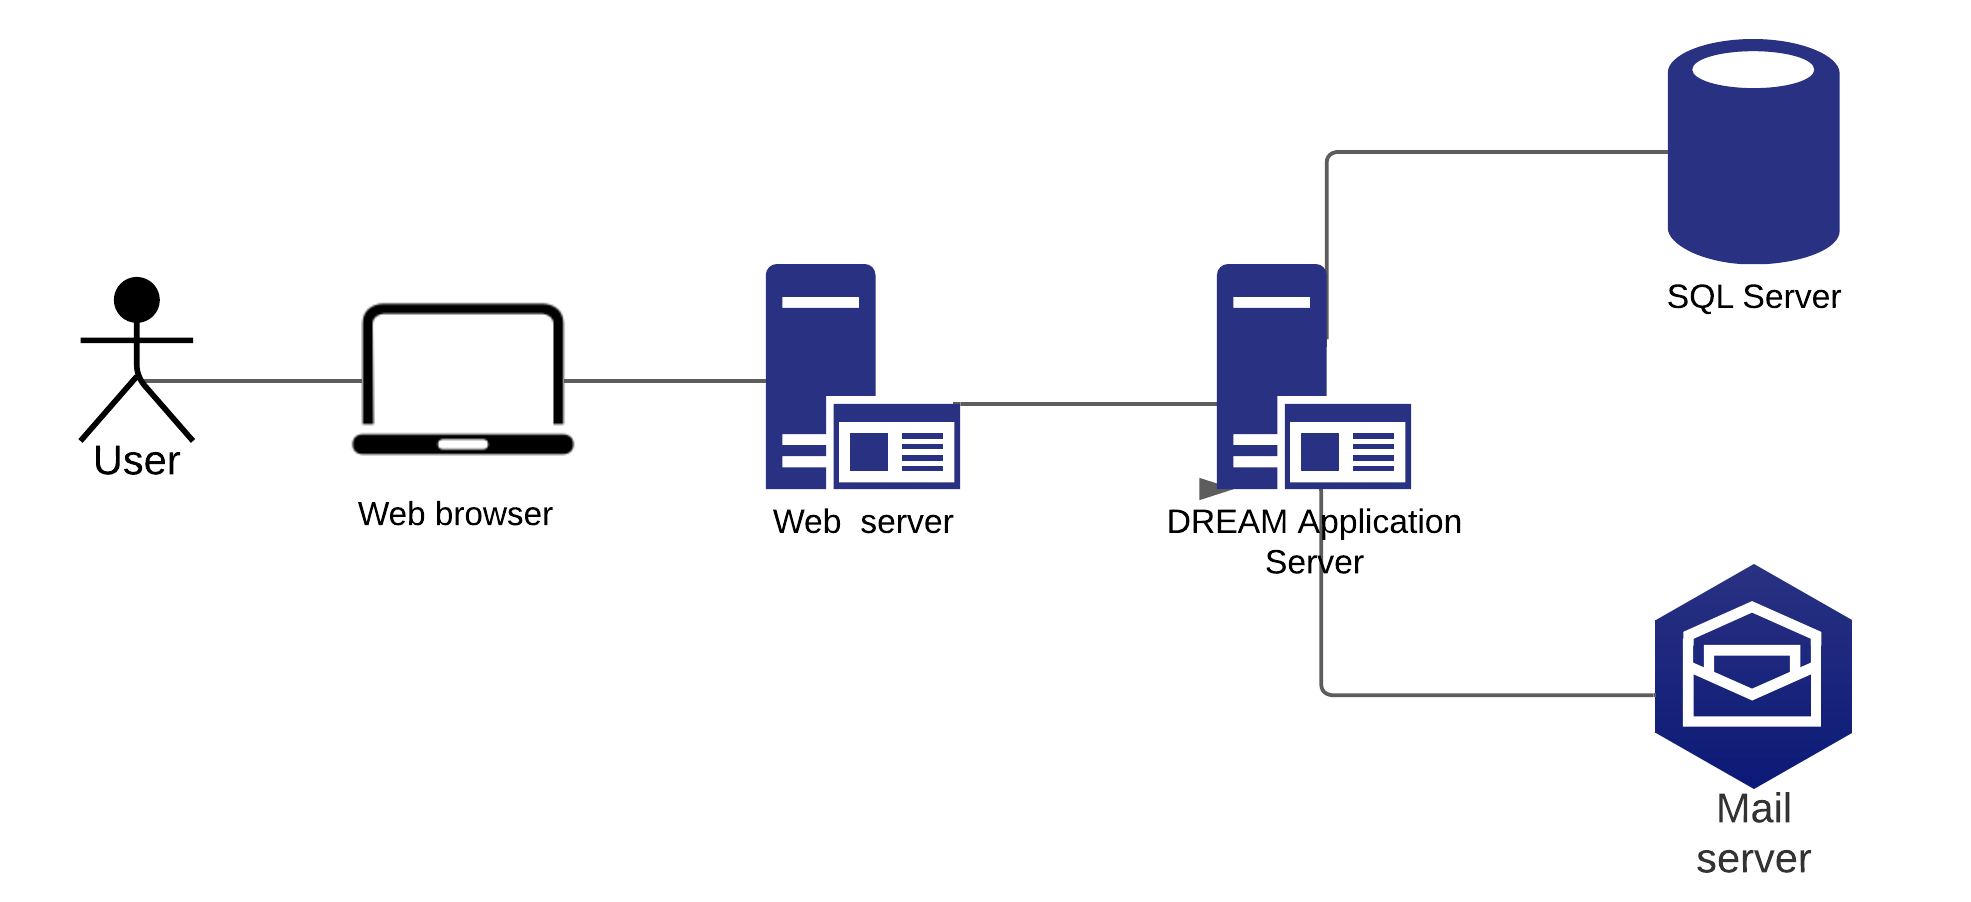
\includegraphics[width=12cm, height=6cm]
    {figures/Overview.png}
    \caption{High-level architecture diagram}
    \label{fig:high-level-architecture}
\end{figure}

The DREAM server part uses a database hosted on a SQL Server to store data collected from the users as well as external systems, and the Mail Server used to send the emails required for password reset. Moreover, the web server works as a middleware between the user interface and the database, utilizing HTTP protocol to receive and respond to requests from the web application running on a client's web browser. Finally, the \textit{DREAM server} hosts the application server (\textit{backend} part) with the majority of the application business logic. 

\section{Component View} \label{sec:component-view}

\subsection{High level}
The following diagram presents a high level overview of the whole DREAM system. It describes both structure of the system and high level interaction within him. The description of the system components, as well as the low level diagram of the application server, are presented below.

\begin{figure}[H]
    \centering
    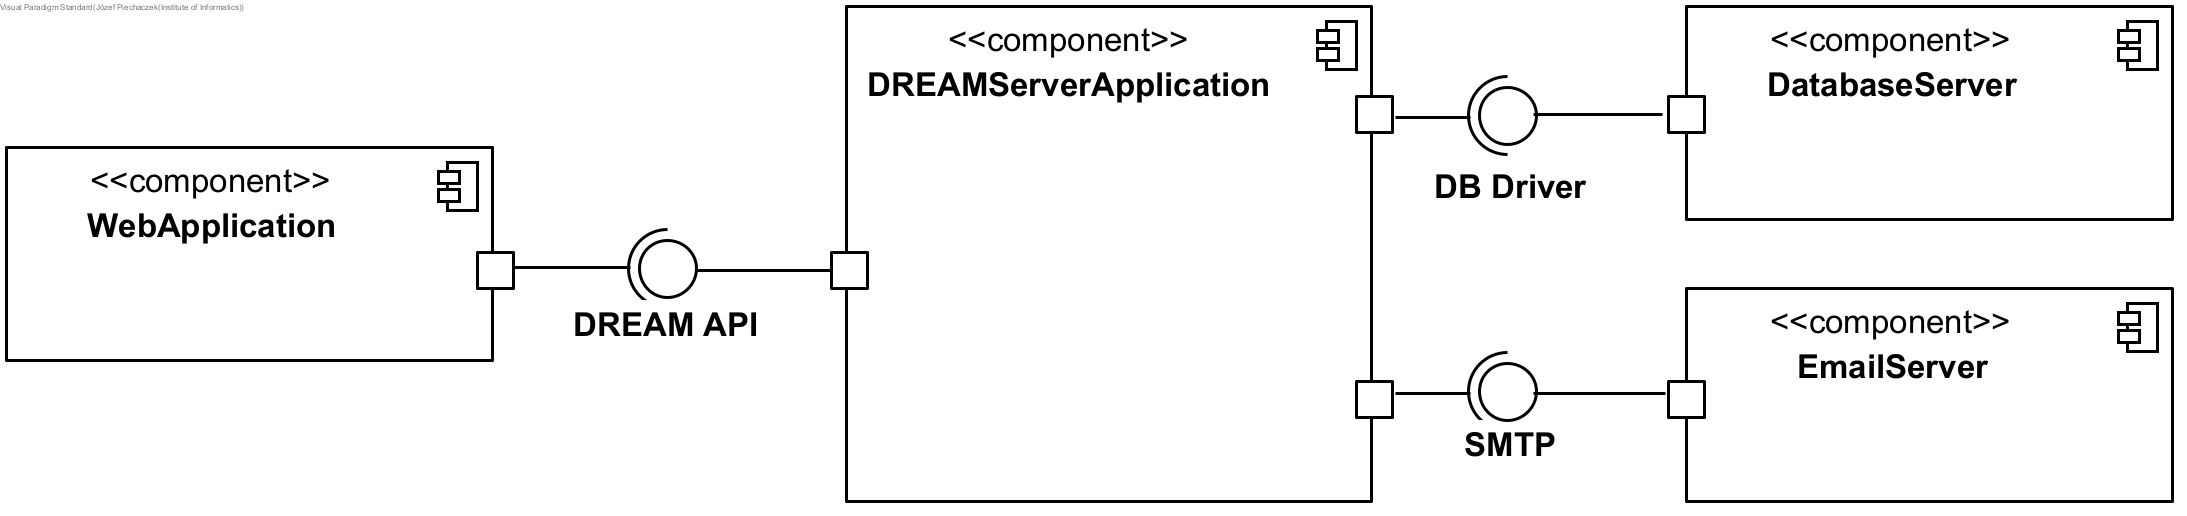
\includegraphics[width=0.85\textwidth]{diagrams/component/High Level Overview.png}
    \caption{DREAM Application high level component diagram}
    \label{fig:high-level-components}
\end{figure}

The system consists of the following components:
\begin{itemize}
    \item \textbf{WebApplication} - frontend part of the application, reachable via any modern browser, regardless of the form factor of the device.
    \item \textbf{DREAMServerApplication} - backend part of the application, handling main application login. It provides a REST API \cite{rest} interface, which is consumed by the WebServer. This component is described in detail in further parts of the document.
    \item \textbf{DatabaseServer} - part of the application responsible for data storage and management. Communicates with DreamServer via a DB Driver.
    \item \textbf{EmailServer} - additional service, allowing system to send a password reminder e-mail using SMTP.
\end{itemize}

\subsection{DREAM server}\label{subsec:backend-components}
Detailed component diagram of the DREAM Server is presented in the figure \ref{fig:backend-components}. The server application was broken down into 3 layers using N-tiers architecture pattern described in section \ref{sec:patterns}. The communication between layers is established by implementation of interfaces presented in the diagram. In accordance with the N-tier pattern, the communication runs only in one direction – starting from the API layer down to the Data Access layer. 

\begin{figure}[H]
    \centering
    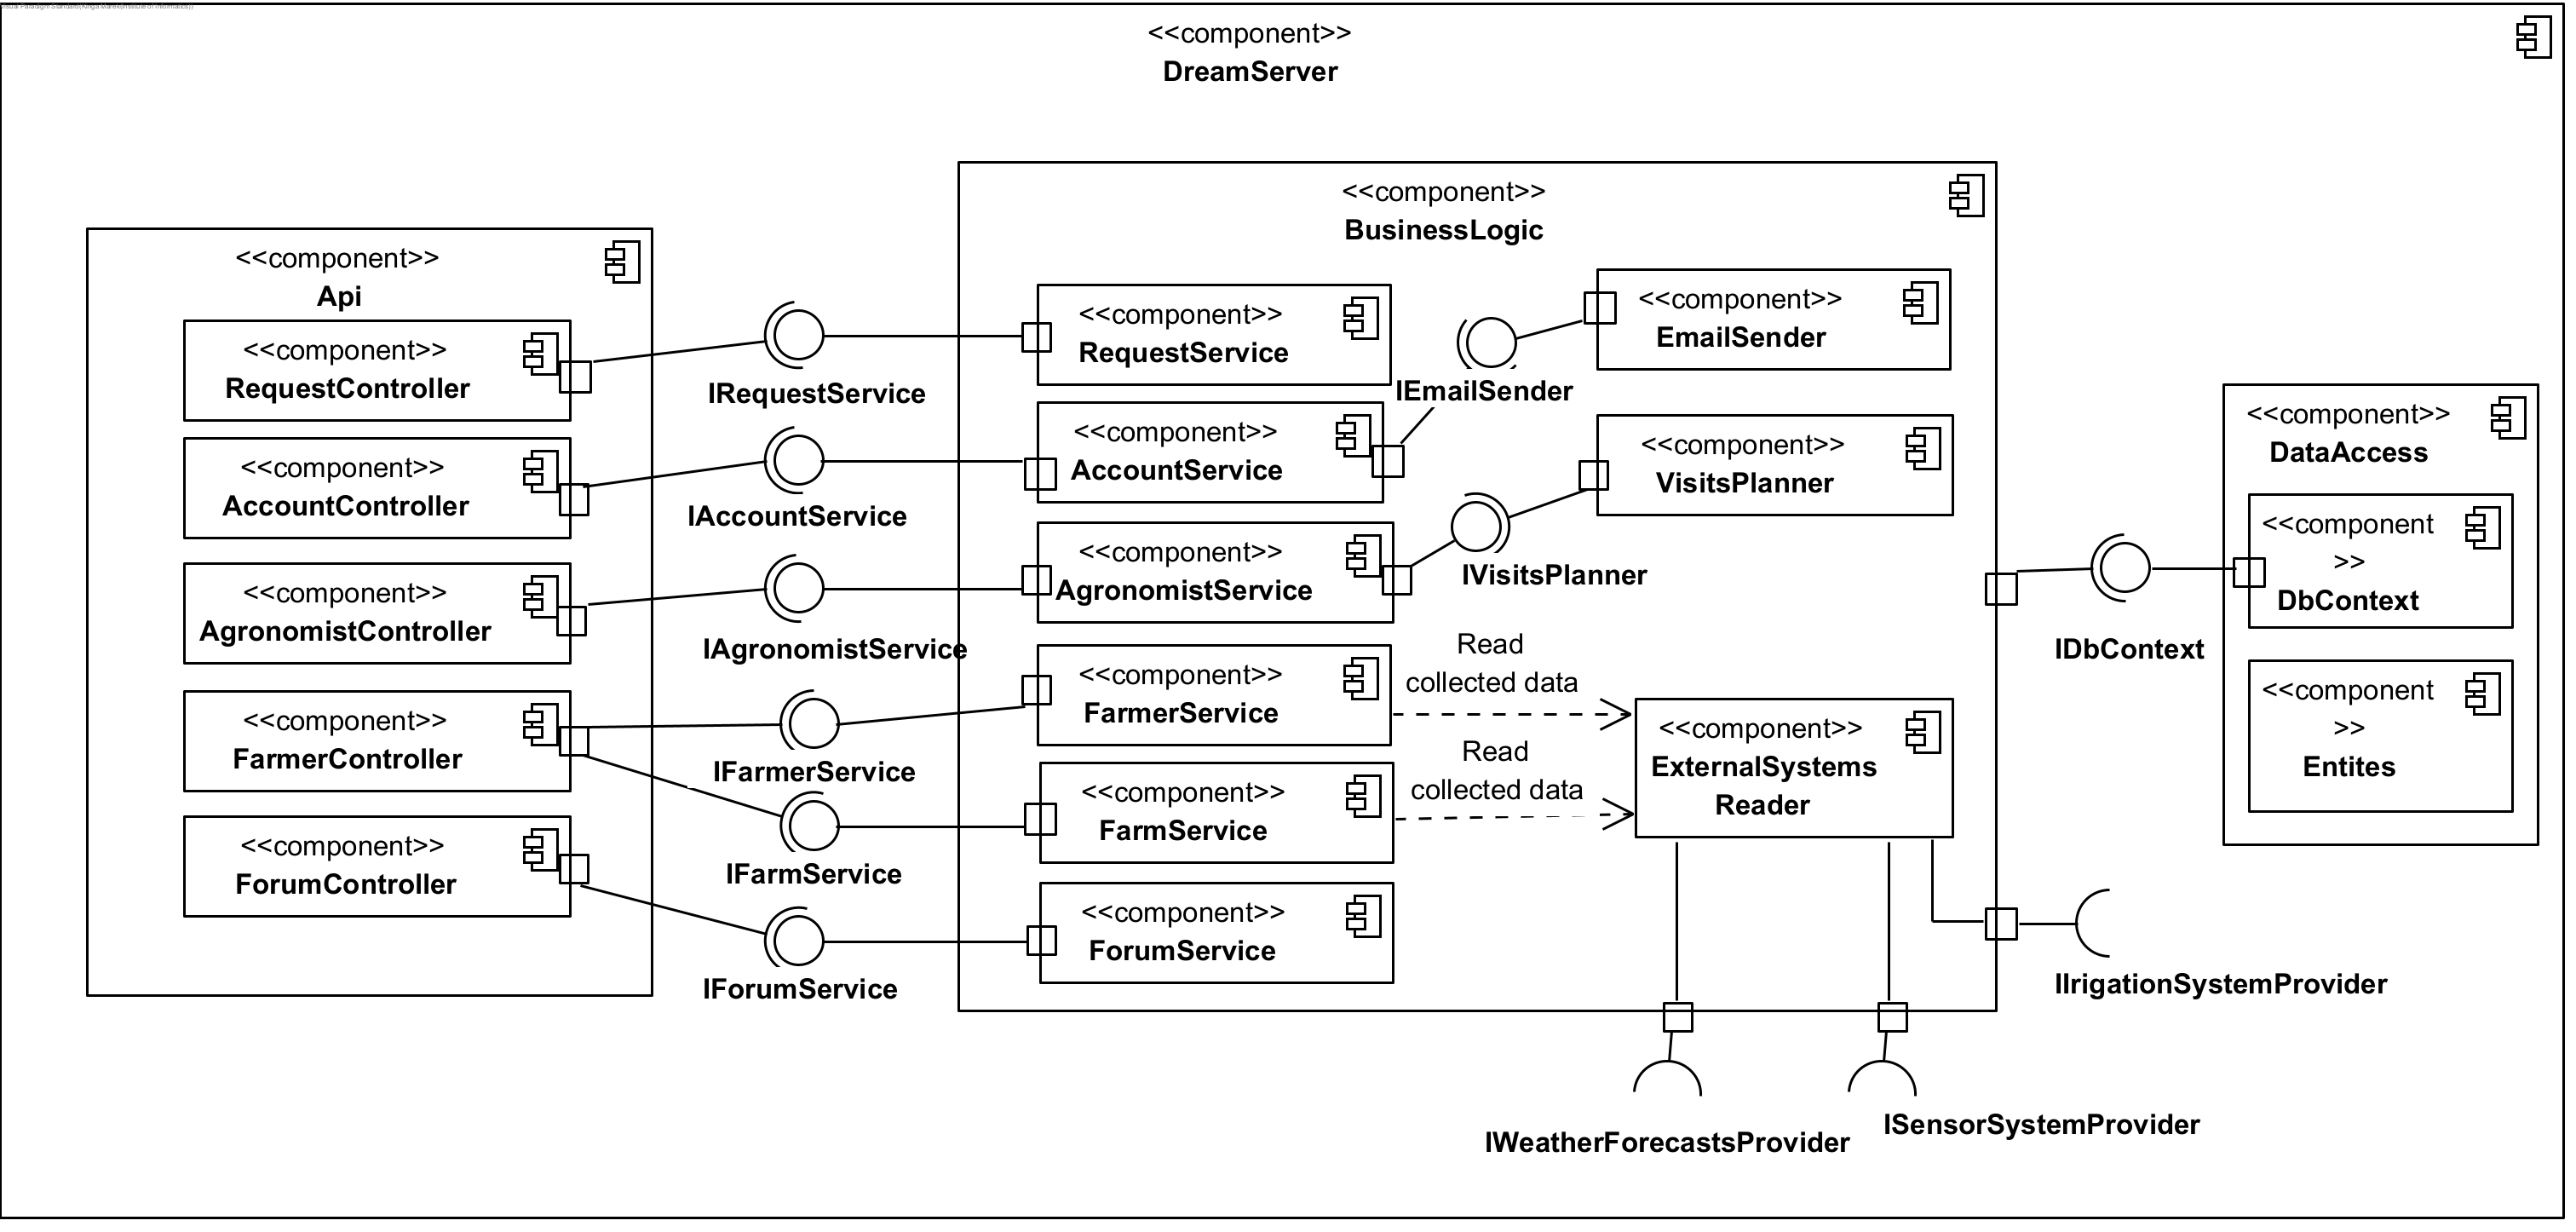
\includegraphics[scale=0.58, origin=c]
    {diagrams/component/BackendComponents.png}
    \caption{DREAM server component diagram}
    \label{fig:backend-components}
\end{figure}

The first layer, the API layer, is composed by a set of controllers that describe available REST endpoints. Then, the middle layer, Business Logic layer contains services and other classes that provide logic necessary for handling HTTP requests  from the client application and cooperation with external systems. In detail, the Business logic layer contains:
\begin{itemize}
    \item \textbf{RequestService} - handles creating, editing, deleting and accessing help requests together with logic required for automatic selection of requests' recipients.
    \item \textbf{AccountService} - handles account registration and deletion, password reset and authentication logic.
    \item \textbf{AgronomistService} - handles area of responsibility and daily plan management, setting execution state of visits. It calls VisistsPlanner about the necessities to plan new visits after each submission of daily plan execution state or rejection of planned visit.
    \item \textbf{FarmerService} - handles notes assignment and providing data required for building farmer's summary (access to notes history). In addition, it allows searching for specified farmer using different query filters. 
    \item \textbf{FarmService} - handles management of farmers' production data, providing data required for building farmer's summary (farm's external systems and  production data).  
    \item \textbf{ForumService} - handles accessing and creating forum threads; accessing, creating and deleting comments.
    \item \textbf{SuggestionService} - handles creating, deleting and reading suggestions by agronomists. Moreover, retrieves personalized suggestions for the farmer based on his farm's location and production type.
    \item \textbf{WeatherForecastService} - handles retrieving different weather forecasts data based on provided query parameters.
    \item \textbf{EmailSender} - handles logic required for e-mail sending during password reset process.
    \item \textbf{VisitsPlanner} - handles implementation of \textit{visits scheduling algorithm} described in subsection \ref{subsec:visits-alg}.
    \item \textbf{ExternalSystemsReader} - handles logic required for execution of daily jobs that read and store in the database data obtained from IWeatherForecastsProvider, ISensorSystemProvider and IIrigationSystemProvider interfaces. The implementation of these interfaces is provided by the external systems' API. 
\end{itemize}

Finally, the Data Access layer contains entities and classes required to efficiently communicate with the database. The components of this layer were not presented in detail, as the communication with the database will leverage object relational mapping, described in more detailed way in the component interfaces section \ref{fig:data-access-interfaces}.

\section{Deployment View}
\begin{figure}[H]
    \centering
    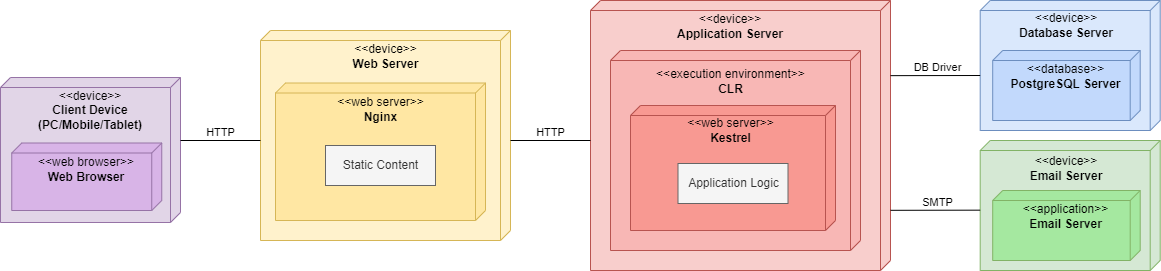
\includegraphics[width=\textwidth]{diagrams/deployment.png}
    \caption{Deployment diagram}
    \label{fig:deployment}
\end{figure}
The system is divided into 5 parts: DREAM Server, Web Server, Database Server, Client Device, and Email Server.
\begin{itemize}
    \item \textbf{DREAM Server} - DREAM backend server, it handles application logic and provides a REST API. It runs using Kestrel Web Server, which is loaded by Common Language Runtime (CLR), the virtual machine component of Microsoft .NET Framework \todo{Missing references}
    \item \textbf{Web Server} - DREAM frontend server, it provides the user interface layer. It hosts the static version of the website using Nginx \cite{nginx}. The website communicates with the Application Server tier via REST API using HTTP requests.
    \item \textbf{Database Server} - Database storage system, using PostgreSQL \cite{postgresql}. It allows data access using DB driver. 
    \item \textbf{Client Device} - Device used by clients to access the website hosted in Web Server tier using HTTP requests. It can be any type of device, capable of running a modern web browser
    \item \textbf{Email Server} - Email server, allowing to send messages via SMTP protocol.
\end{itemize}

\section{Runtime View}

The sequence diagrams presented in this chapter illustrate the application's runtime perspective. They define how components (introduced in the section \ref{sec:component-view}) interact with one another to realize the DREAM's most essential use cases in a more detailed way than it was depicted in RASD. The diagrams assume that requests sent to \textit{DbContext} are always handled correctly (which cannot be guaranteed), so that their complexity does not expand dramatically.

\subsection*{Create account}

The ability to create a user account is the most essential functionality provided by the system. As already mentioned in RASD, DREAM provides three types of actors: agronomists, farmers, and policy makers. The registration data varies depending on the chosen role, i.e. every agronomist must specify his area of responsibility, whereas every farmer needs to provide data regarding his farm. All of this is handled via the \textit{WebApplication} component. Subsequently, \textit{AccountController} forwards the request to \textit{AccountService}, which interacts directly with \textit{DbContext}. Moreover, when a farmer creates his account, \textit{AccountService} ensures that both a farm and two casual visits are created instantly, thus satisfying the requirement \textbf{R5}. The whole process is presented in the figure \ref{fig:sd_create_account}.

\begin{figure}
    \centering
    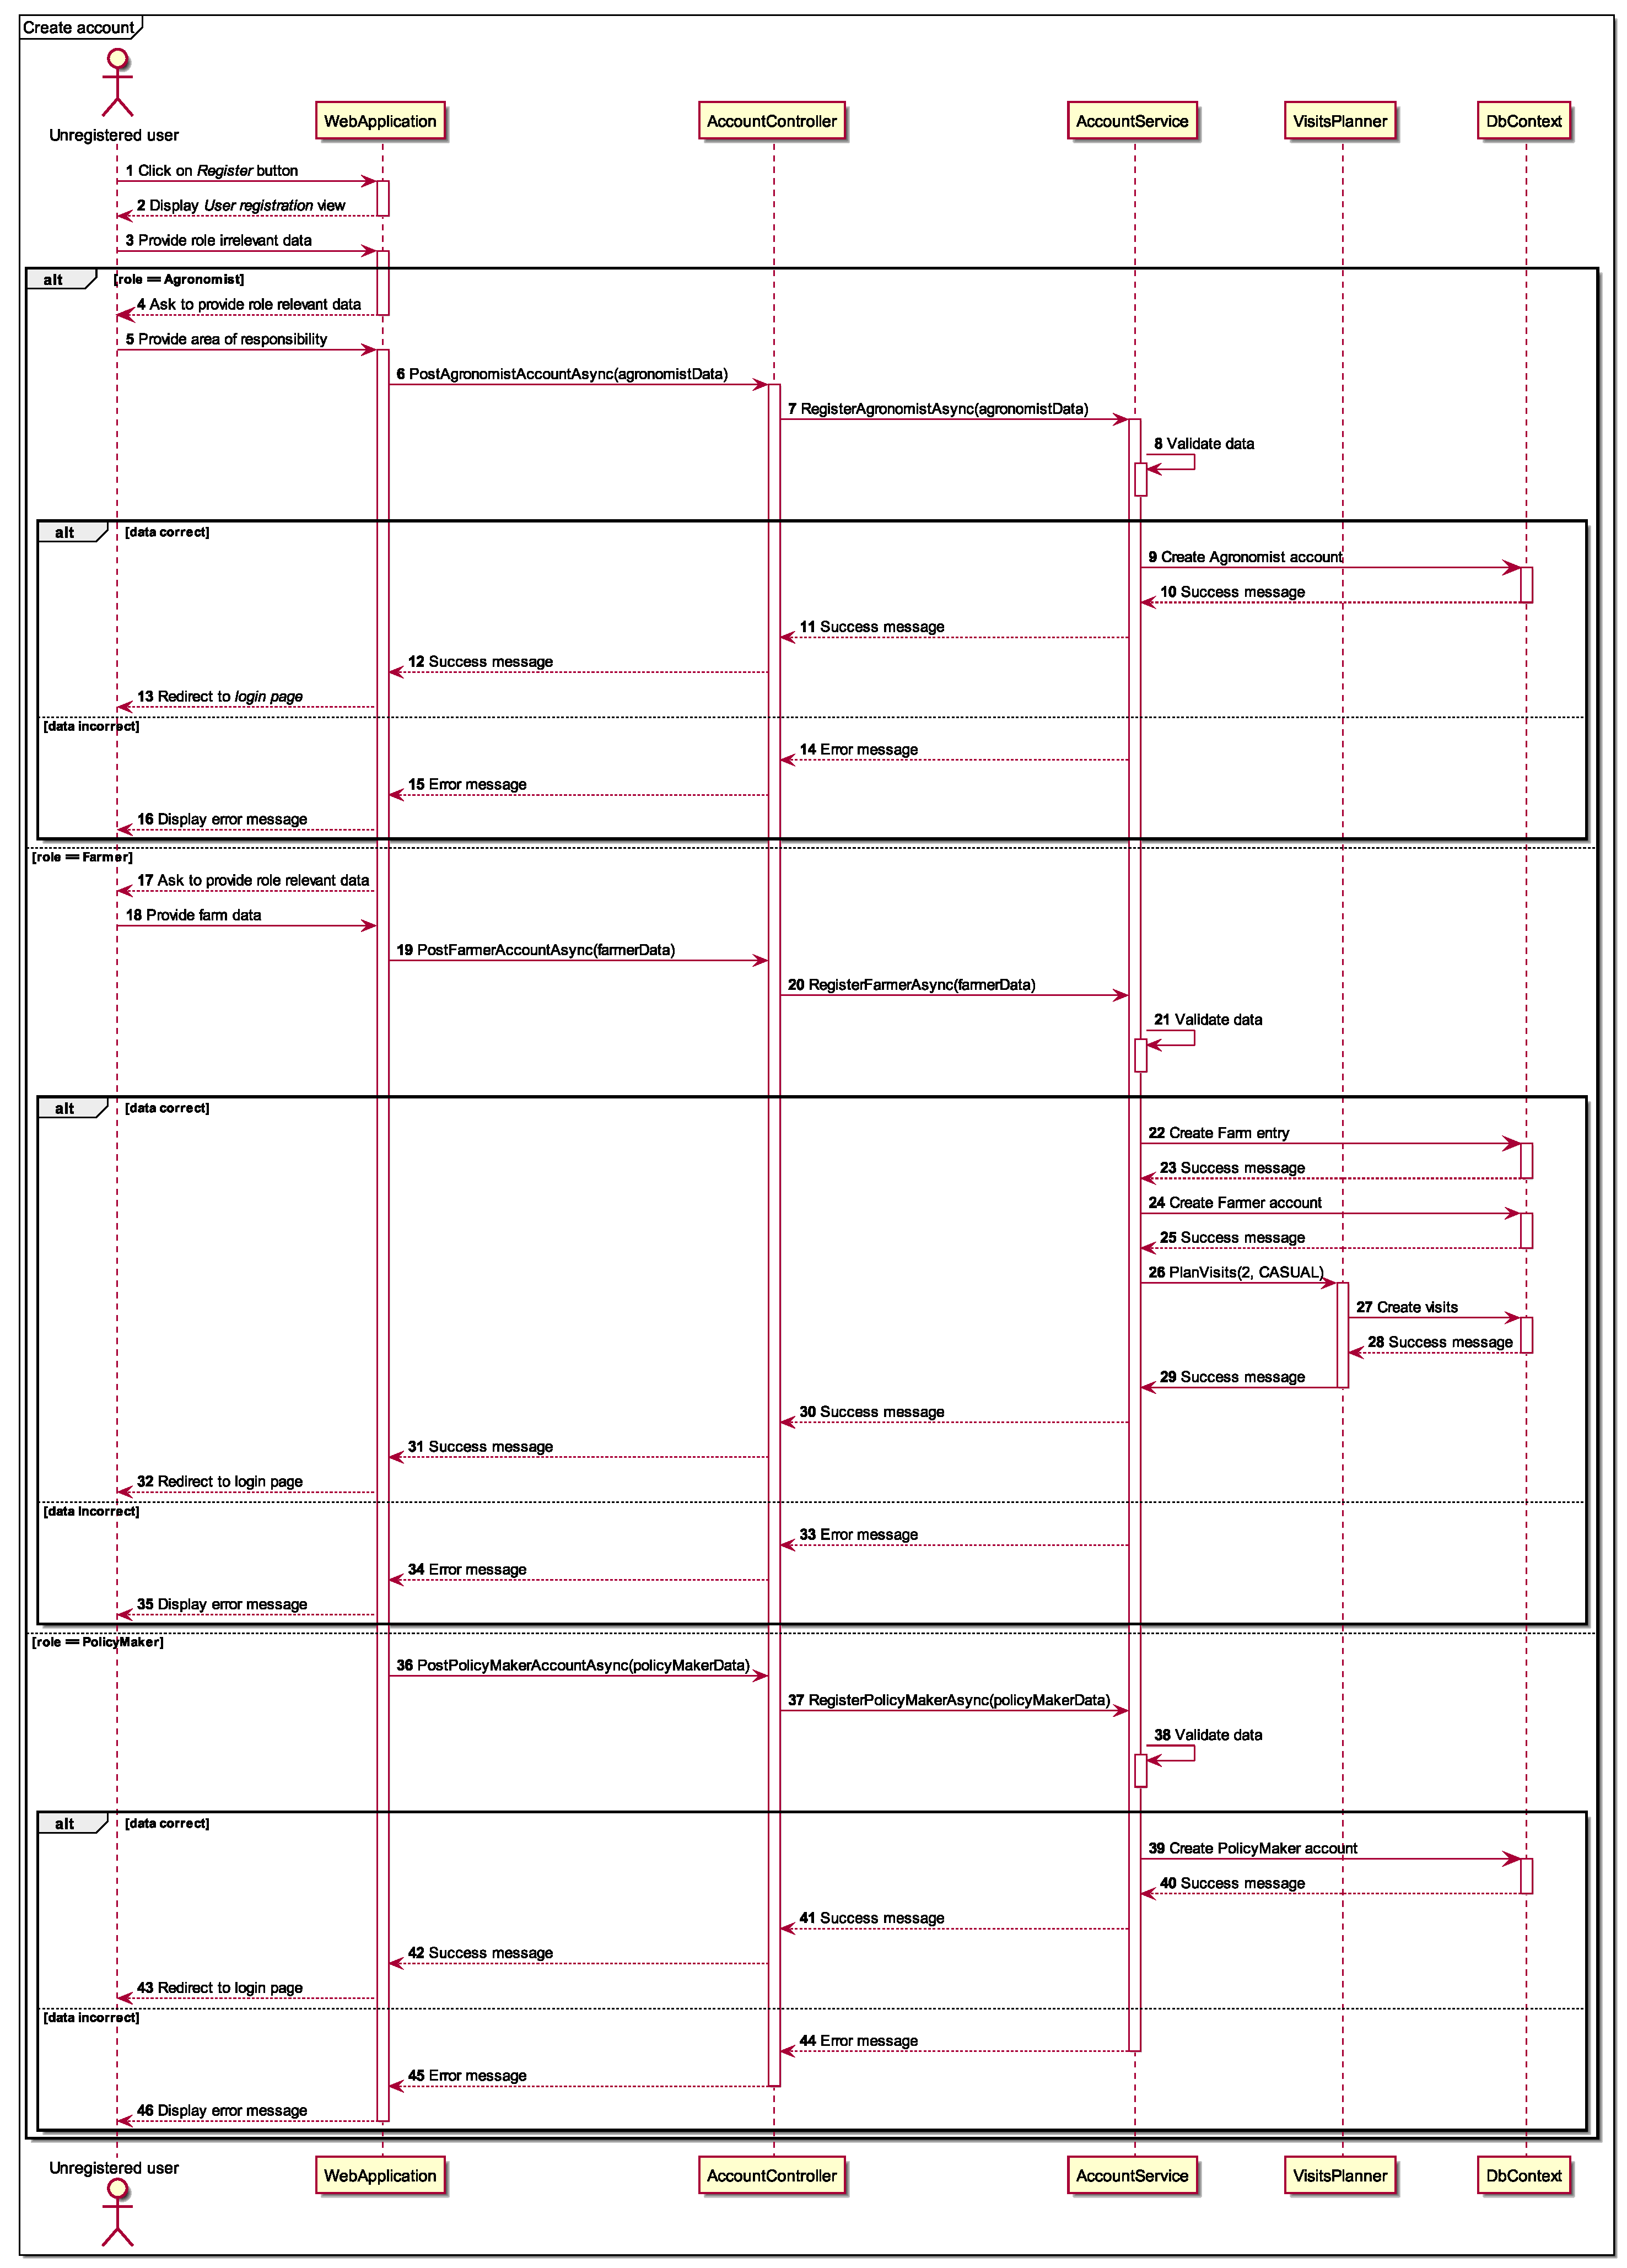
\includegraphics[height=\textheight, width=\textwidth, keepaspectratio, origin=c]{diagrams/sequence/create_account}
    \caption{Sequence diagram presenting the process of creating a new user account.}
    \label{fig:sd_create_account}
\end{figure}

\subsection*{Request help}

The sequence diagram displayed in the figure \ref{fig:sd_request_help} shows the process of creating a help request by the farmer. After specifying its topic and contents, \textit{WebApplication} forwards that data to \textit{RequestController}, which then interacts with \textit{DbContext} via \textit{RequestService}. Correctly created help request is displayed to the farmer afterwards.

\begin{figure}
    \centering
    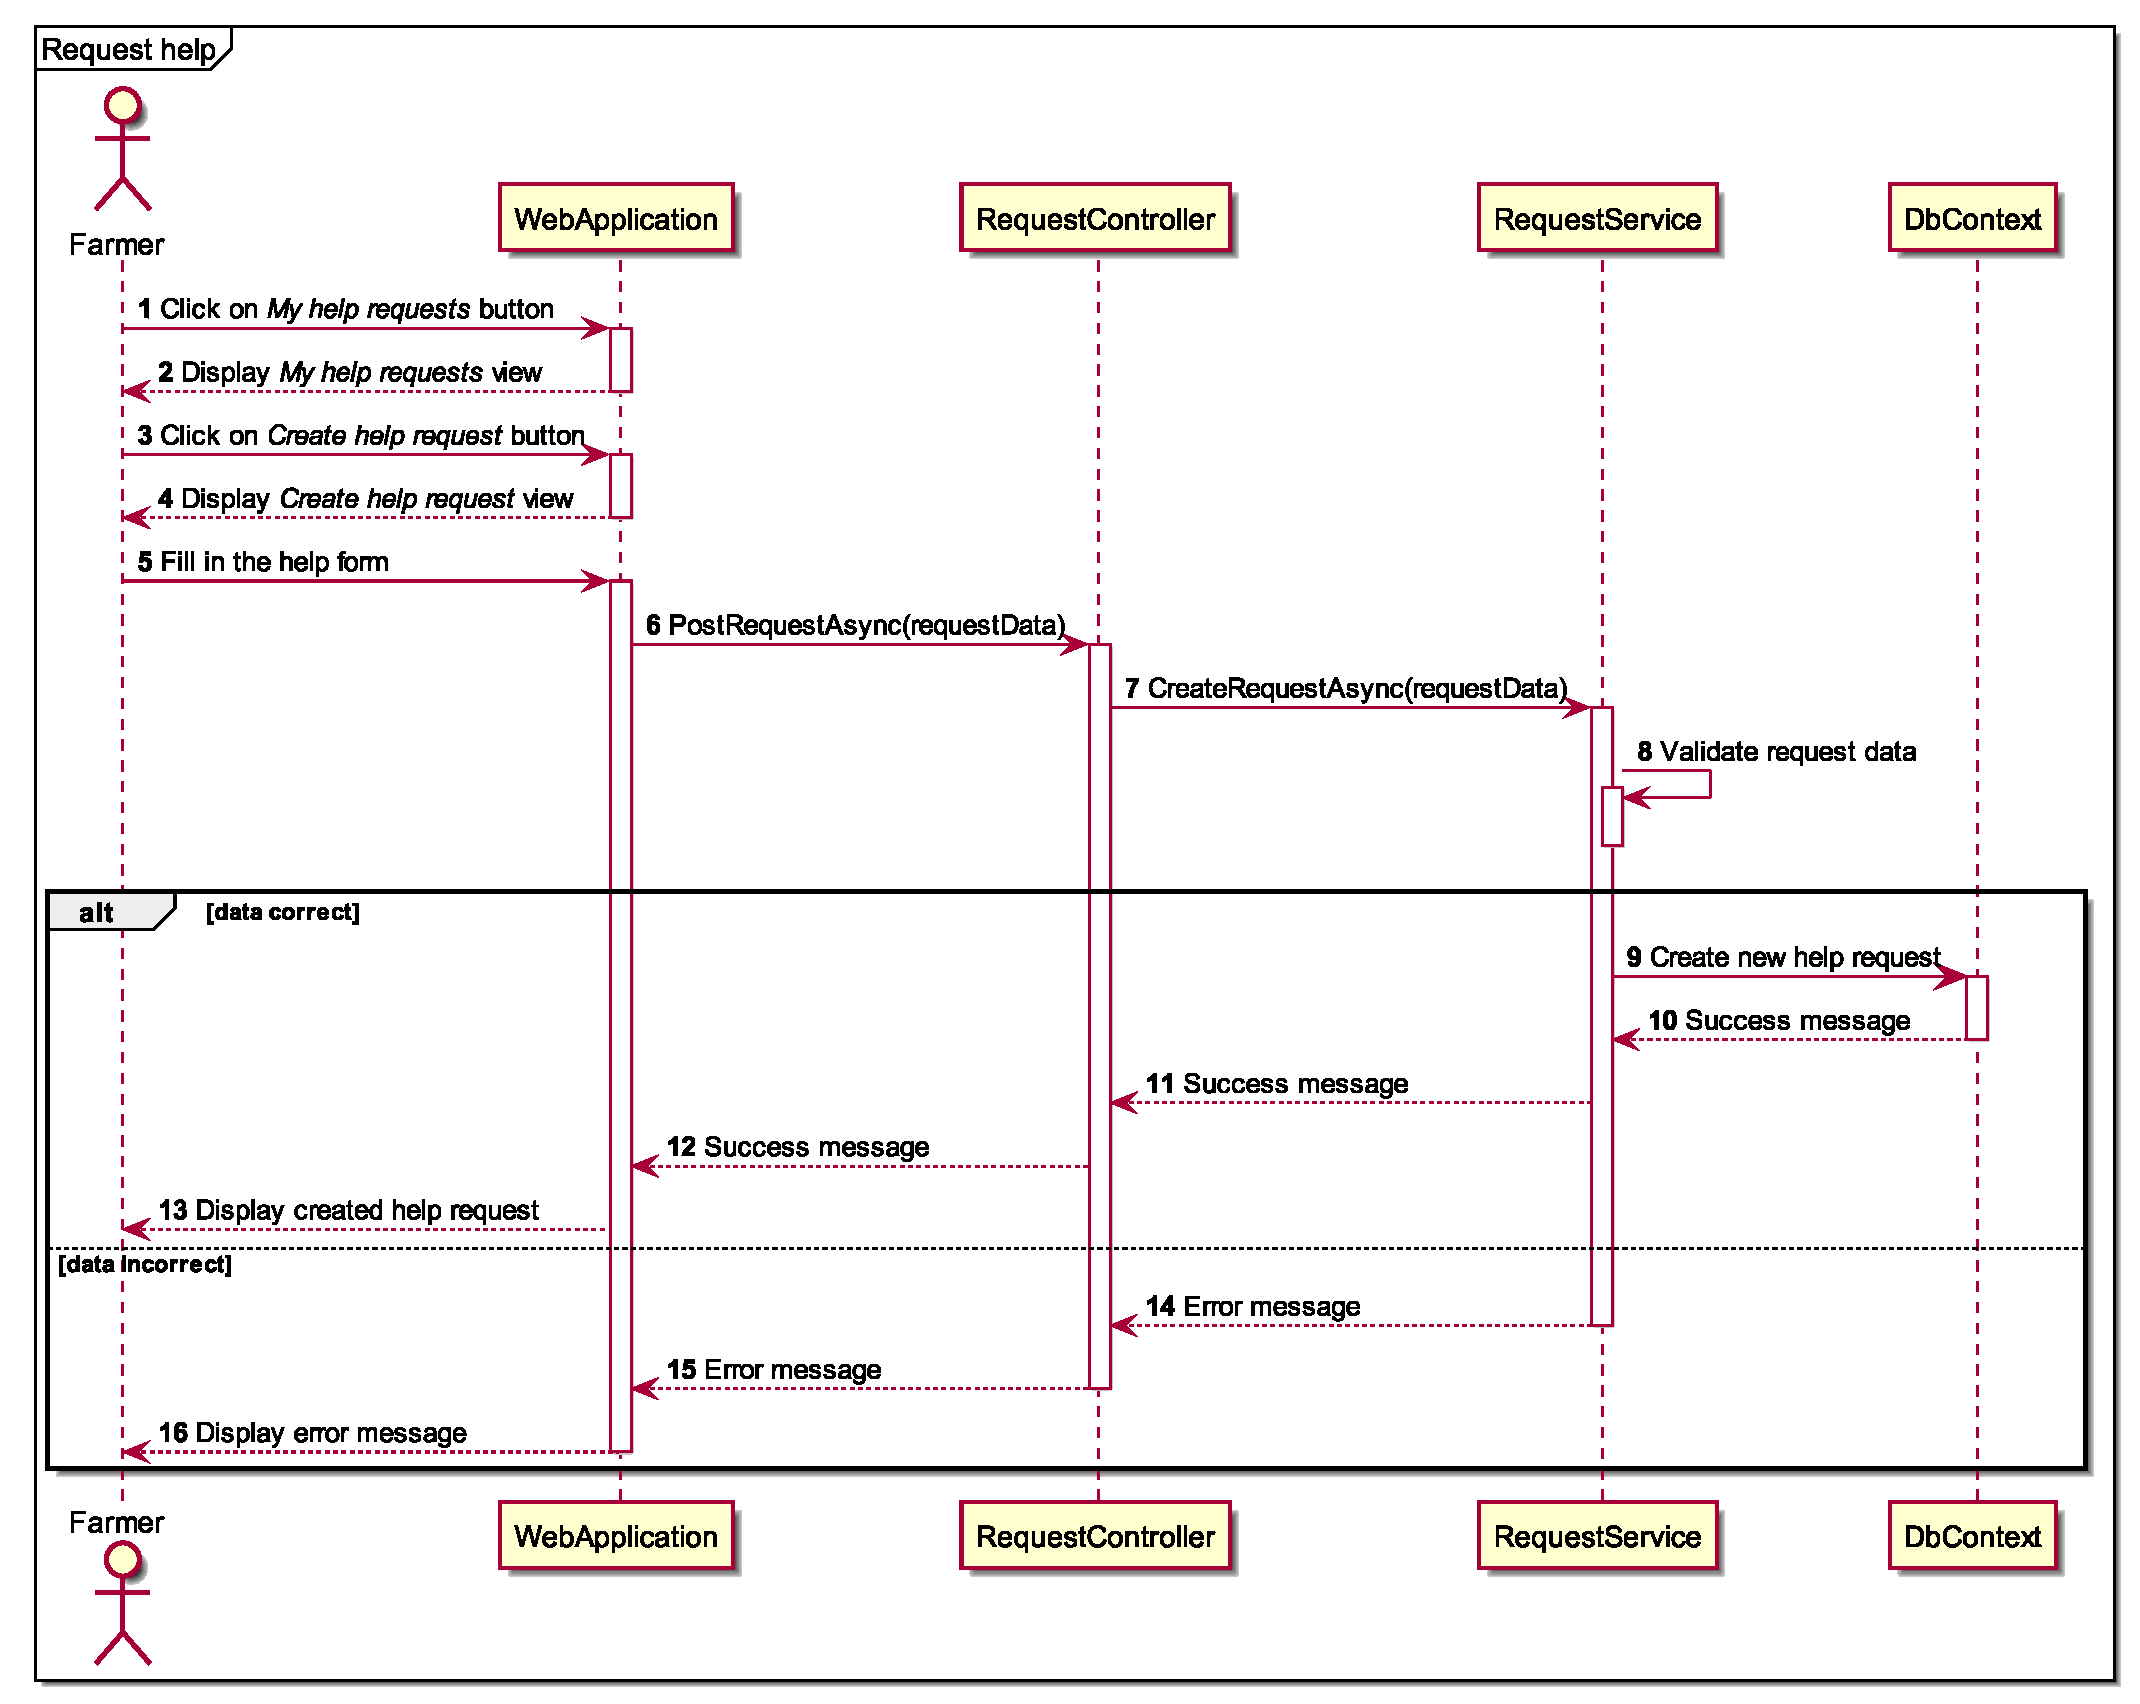
\includegraphics[height=\textheight, width=\textwidth, keepaspectratio, origin=c]{diagrams/sequence/request_help}
    \caption{Sequence diagram presenting the creation of a help request.}
    \label{fig:sd_request_help}
\end{figure}

\subsection*{Assess farmer's performance}

Giving policy makers the possibility to assess farmers' performance is one of the most important functionalities of DREAM. It takes a coordination of the following components to fulfill this use case: \textit{WebApplication}, \textit{FarmerController}, \textit{FarmerService}, \textit{RequestController}, \textit{RequestService}, \textit{VisitsPlanner}, and \textit{DbContext}. Furthermore, supplementary collaboration of \textit{FarmService}, \textit{WeatherForecastController}, and \textit{WeatherForecastService} is required in order to construct the farmer's summary. The diagram presented in the figure \ref{fig:sd_assess_farmers_performance} provides a thorough description of this process. It leverages the visit scheduling algorithm (see section \ref{subsec:visits-alg}) to satisfy the requirements \textbf{R17} and \textbf{R18}.

\begin{figure}
    \centering
    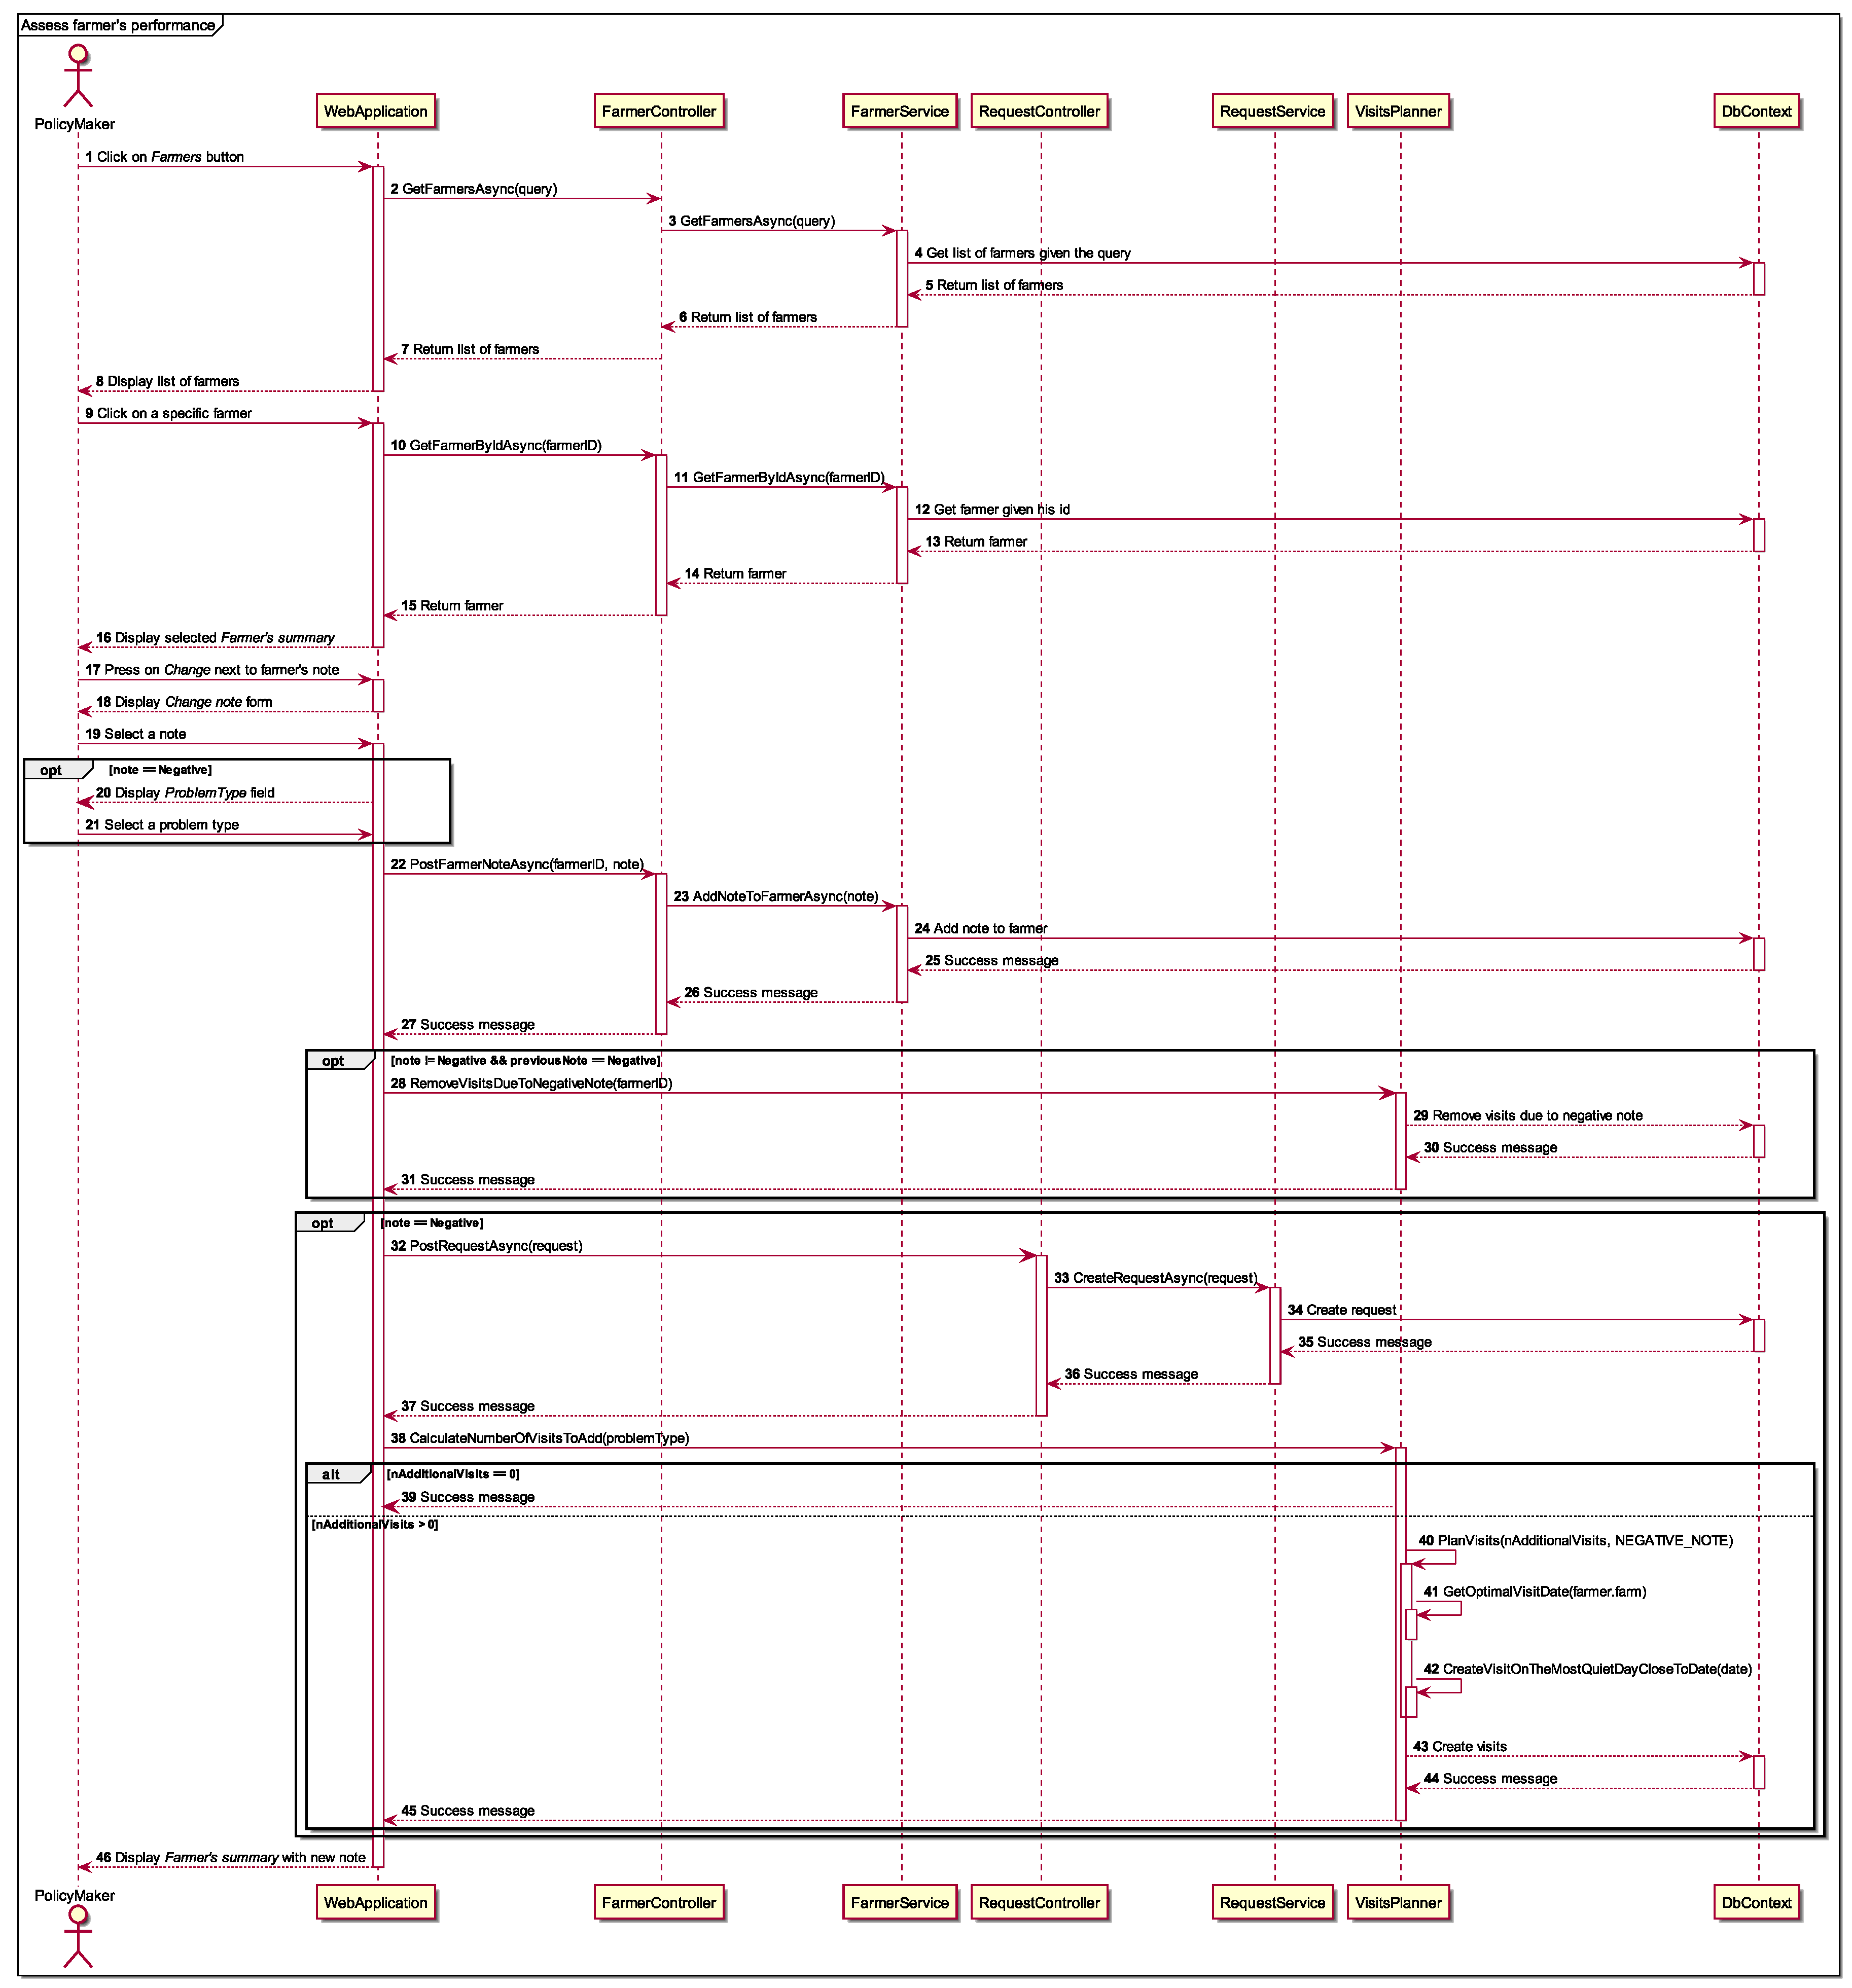
\includegraphics[height=\textheight, width=\textwidth, keepaspectratio, origin=c]{diagrams/sequence/assess_farmers_performance}
    \caption{Sequence diagram presenting farmer's performance assessment.}
    \label{fig:sd_assess_farmers_performance}
\end{figure}

\subsection*{Set execution state of a daily plan}

In the agricultural field, an agronomist acts as a liaison between farmers and policymakers. He provides advice on soil management and productivity to farmers. In the Telangana region, government agronomists visit farms in their areas of responsibility on a regular basis to gather information about farmers' performance. Thus, a possibility to organize all the appointments inside one interactive schedule is a vastly desired feature. It is realized via several components including \textit{WebApplication}, \textit{AgronomistController}, \textit{AgronomistService}, \textit{VisitsPlanner}, and \textit{DbContext}. The interactions between them are depicted in the figure \ref{fig:sd_set_daily_plan_execution_state}.

\begin{figure}
    \centering
    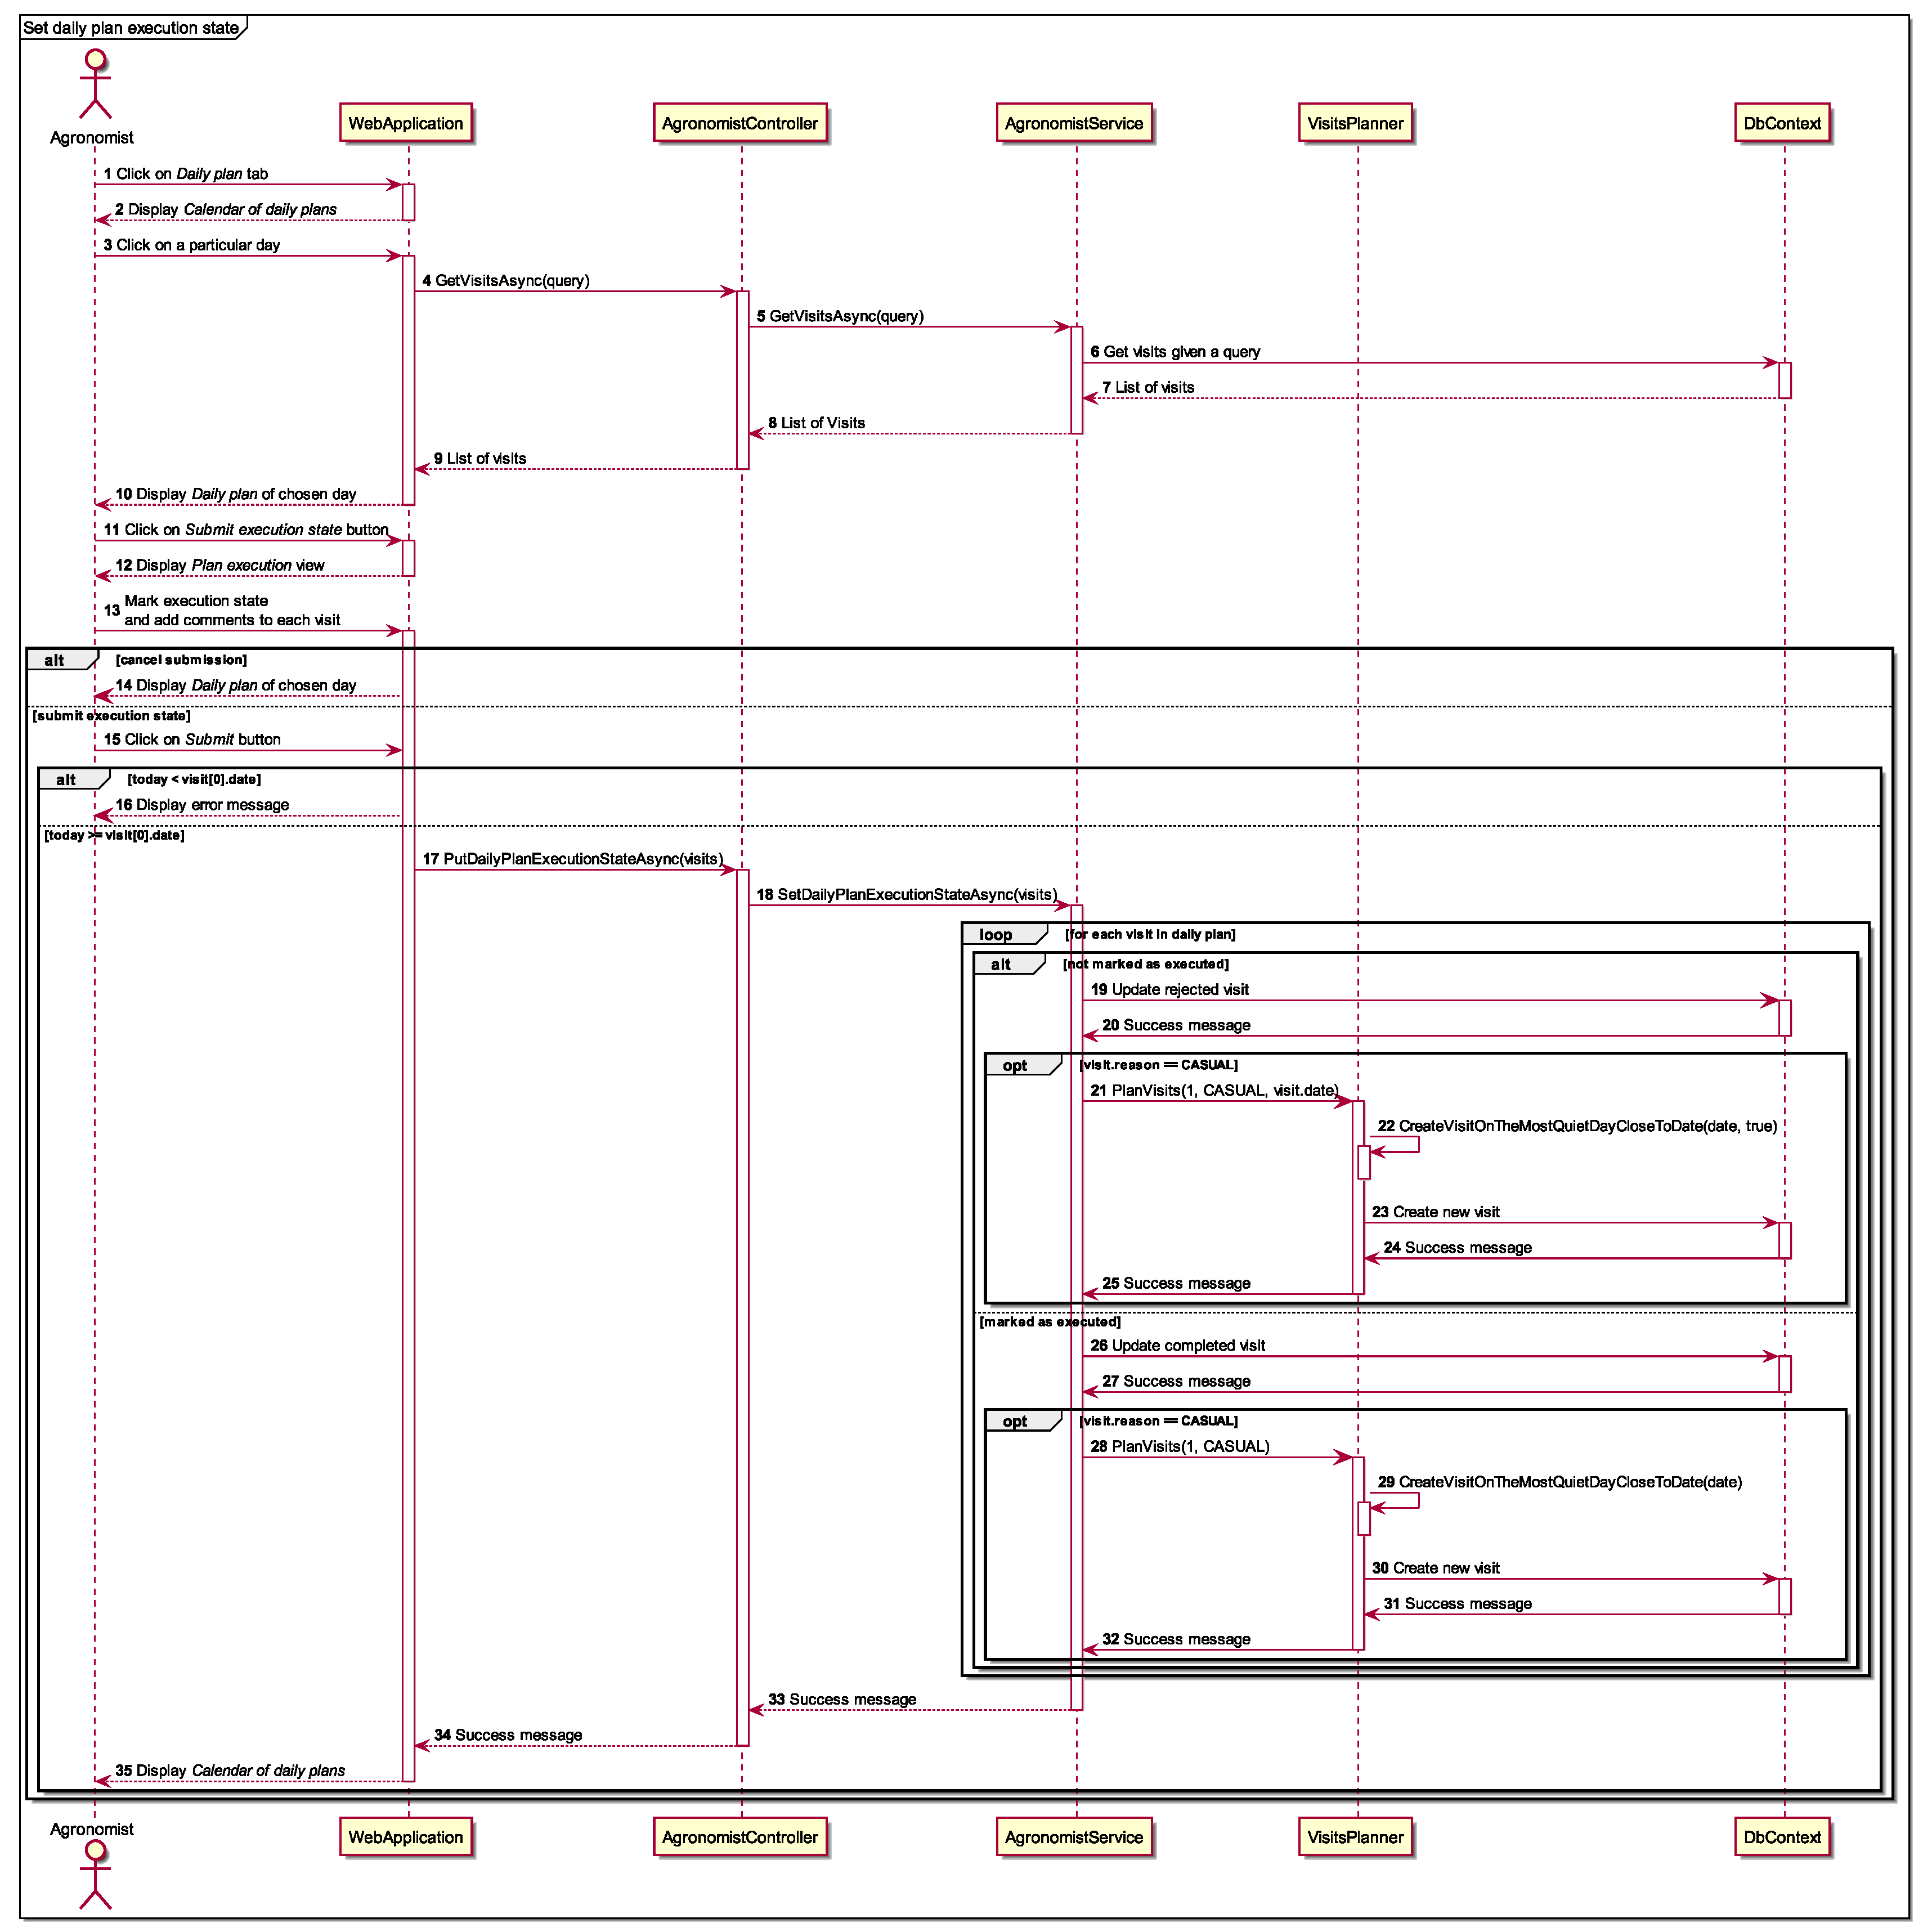
\includegraphics[height=\textheight, width=\textwidth, keepaspectratio, origin=c]{diagrams/sequence/set_daily_plan_execution_state}
    \caption{Sequence diagram presenting the action of displaying a daily plan.}
    \label{fig:sd_set_daily_plan_execution_state}
\end{figure}

\section{Component Interfaces}
The figures in this chapter depict methods implemented by the components of the DREAM server application presented previously in the figure \ref{fig:backend-components}.

\begin{figure}[H]
    \centering
    \includegraphics
    [width=\textwidth]
    %[scale=0.75, origin=c]
    {diagrams/component/API-interfaces.png}
    \caption{API components' interfaces}
    \label{fig:api-interfaces}
\end{figure}

The first figure (\ref{fig:api-interfaces}) represents controllers provided by the API layer to define HTTP endpoints exposed by the DREAM application server. 

\begin{figure}[H]
    \centering
    \includegraphics
    [width=\textwidth]
    %[scale=0.75, origin=c]
    {diagrams/component/BusinessLogic-interfaces.png}
    \caption{Business Logic components' interfaces}
    \label{fig:business-logic-interfaces}
\end{figure}

The second figure (\ref{fig:business-logic-interfaces}) presents interfaces that the components of the business logic layer implement. Specifically, the interfaces contain methods responsible for areas described in section (\ref{subsec:backend-components}) where DREAM server application components are presented. One of the implementation conventions that can be spotted here and in the previous figure is the use of \textit{async} suffix for naming asynchronous methods in C\#. It is an asynchronous design pattern recommended by Microsoft \cite{async}. 

\begin{figure}[H]
    \centering
    \includegraphics
    [width=\textwidth]
    %[scale=0.75, origin=c]
    {diagrams/component/DataAccess-interfaces.png}
    \caption{Data Access components' interfaces}
    \label{fig:data-access-interfaces}
\end{figure}

The last figure \ref{fig:data-access-interfaces} shows the classes of the Data Access layer. However, the details of classes presented in the figure are not shown to preserve readability. Those classes (apart from DreamDbContext class) do not contain any methods, since they serve for object-relational mapping \cite{ef}.  Hence, each of them corresponds to at least one table in the database diagram (more than one in case of many-to-many relationships). Similarly, the fields of those classes correspond to the tables' columns. Detailed database diagram is presented in the following sections, in the figure \ref{fig:db-model}. The only class that contains logic in this figure is the DreamDbContext. It acts as a bridge between the database and the C\# code – it contains fields that represent the tables of the database \cite{ef-dbcontext}.


\section{Selected Architectural Styles and Patterns}\label{sec:patterns}
\begin{itemize}
    \item \textbf{Client Server} - a pattern, which enforces the principle of separation of concerns, by separating the service requesters (clients) from the providers of a resource or service (servers). Clients and servers communicate over a network and can be hosted on separate hardware.
    \item \textbf{REST} (\textit{Representational State Transfer}) – the API hosted on a DREAM server should be prepared using the REST API design rules \cite{rest} \cite{rest-microsoft}. Firstly, it should not bind the client application to any specific implementation by utilizing HTTP as the communication protocol. Furthermore, as it was presented in the DREAM server components diagram in subsection \ref{subsec:backend-components}, additional layers will be introduced to the server side application to avoid direct dependencies of the API on the database model. Additionally, the interface should be resource-oriented and the HTTP methods \cite{rfc1945} should reflect the operations done on the resources. All this aims at improving the maintainability, reusability, and readability of the server application.
    \item \textbf{N-tier application} – the server side application was divided into 3 layers: API, Business Logic, and Data Access. This architecture was adopted following the types of common web application architectures described in Microsoft's documentation \cite{ntier}. However, the \textit{User Interface} layer was replaced by \textit{API} layer to better present its meaning. The choice was motivated by the simplicity of the architecture compared to other architectures like \textit{Clean architecture} or microservices architecture. 
    \item \textbf{Dependency Injection} - a dependency inversion technique that focuses on providing the implementation of required interfaces instead of creating them explicitly by the dependent objects \cite{di}. The main reason for introduction of this principle is the need to address the difficulty of testing the business logic layer \cites{ntier}. \todo{move it to the implementation chapter?}
\end{itemize}

\section{Other Design Decisions}

\subsection{Visit Scheduling Algorithm}\label{subsec:visits-alg}

One of the most important features of the system is the ability to schedule agronomist's visits to a farm. Requirement \textbf{R5} (all the requirements are described in RASD) states that all farms must be visited at least twice a year, whereas \textbf{R14} extends it further by adding a constraint that under-performing farmer's, meaning farmers with a negative note, should be visited more often, depending on the problem they are facing.

The system must be therefore able to schedule visits to a farm in a way that satisfies both requirements. This section presents an overview of the algorithm employed to tackle this problem. All the listings provided include pseudocode that is intended to demonstrate only the high-level notion.

\subsubsection*{General approach}

When planning a new visit it is necessary to take the following factors into consideration:
\begin{itemize}
    \item dates and number of already planned visits to the farm,
    \item number of visits planned for an agronomist on a given day,
    \item type of the problem the farmer is facing.
\end{itemize}

Function \textit{calculateVisitsToAdd} presented in the listing \ref{lst:CalculateVisitsToAdd} calculates the number of visits to add to the farm, given the number of already planned visits to the farm, the number of visits planned for an agronomist on a given day and the type of the problem the farmer is facing. In case there are already more visits to the farm planned than the number of casual visits (2) and the number of visits to add, then no new visit is necessary and the function returns 0. Such situation may happen when there are many visits planned to one farm due to the agronomist's decision.

\lstinputlisting[language=Cpp, caption={Function calculating the number of visits to add due to a problem.}, label={lst:CalculateVisitsToAdd}]{algorithms/visit_scheduling/CalculateVisitsToAdd.cpp}

Another function, presented in the listing \ref{lst:GetOptimalVisitDate} is \textit{getOptimalVisitDate}. It finds the greatest gap between two consecutive visits to the farm and inserts a new visit in between. It also considers a time slot in exactly one year from the current date, so that in case of completing a casual visit, a new one is created in approximately half of a year.

\lstinputlisting[language=Cpp, caption={Function responsible for picking the optimal date of a new visit.}, label={lst:GetOptimalVisitDate}]{algorithms/visit_scheduling/GetOptimalVisitDate.cpp}

\subsubsection*{Planning additional visits}

This section presents the process of scheduling a new visit to a farm. Function \textit{createVisitOnTheMostQuietDayCloseToDate} is presented in the listing \ref{lst:CreateVisitOnTheMostQuietDayCloseToDate}. It is responsible for creating a new visit to the farm on the most quiet day close to the date specified in the function's argument. It goes through up to 5 days before the proposed date and searches for an agronomist, who has not reached the maximum number of visits to the farm on a given day, otherwise, the visit is scheduled for the agronomist with the least visits planned in the specified window.

\lstinputlisting[language=Cpp, caption={Function creating a new visit on the most quiet day that is close to the specified date.}, label={lst:CreateVisitOnTheMostQuietDayCloseToDate}]{algorithms/visit_scheduling/CreateVisitOnTheMostQuietDayCloseToDate.cpp}

Function \textit{createAdditionalVisits}, presented in the listing \ref{lst:CreateAdditionalVisit}, is the main function responsible for scheduling additional visits to the farm.

\lstinputlisting[language=Cpp, caption={Function creating additional visits.}, label={lst:CreateAdditionalVisit}]{algorithms/visit_scheduling/CreateAdditionalVisit.cpp}

Due to the abovementioned requirements, the system must be able to schedule different types of visits to the farm. These types are identified by the visit's reason. The following listing \ref{lst:PlanVisits} presents the function meant to handle this problem.

\lstinputlisting[language=Cpp, caption={Function responsible for planning new visits.}, label={lst:PlanVisits}]{algorithms/visit_scheduling/PlanVisits.cpp}

\subsubsection*{Farmer registration}

Listing \ref{lst:CreateFarmer} presents the process of creating a farmer. Each time a new farmer is created, the system must plan two casual visits to his farm.

\lstinputlisting[language=Cpp, caption={Function responsible for creating a new farmer.}, label={lst:CreateFarmer}]{algorithms/visit_scheduling/CreateFarmer.cpp}

\subsubsection*{Daily plan submission}

Function \textit{updateVisit} (listing \ref{lst:UpdateVisit}) is responsible for changing the date of a visit. It is only possible to do so only if the new date is greater or equal than the current one. In case an agronomist wants to reschedule a visit that is casual, the system allows him to do so, but the date can be postponed only by a maximum of 5 days. Otherwise, the systems rejects the request and throws a warning.

\lstinputlisting[language=Cpp, caption={Function responsible for updating a visit.}, label={lst:UpdateVisit}]{algorithms/visit_scheduling/UpdateVisit.cpp}

The process of submitting a visit is described in the listing \ref{lst:SubmitVisit}. In case the date of a visit is greater than the current date, the visit is submitted. In case the date is less than the current date, a warning is thrown. A casual visit is a cyclic one, therefore a new one is scheduled every time its status becomes confirmed or rejected. In case of rejecting a casual visit, a new one is scheduled in the maximum of next 5 days following the process shown in the listing \ref{lst:PlanVisits}.

\lstinputlisting[language=Cpp, caption={Function responsible for submitting a visit.}, label={lst:SubmitVisit}]{algorithms/visit_scheduling/SubmitVisit.cpp}

\subsubsection*{Obtaining a negative note}

Every time a farmer's note changes from negative to neutral or positive, the system deletes all the visits to the farm that were planned due to the negative note. The function \textit{DeleteVisitsCreatedDueToNegativeNote} (listing \ref{lst:DeleteVisitsCreatedDueToNegativeNote}) handles that.

\lstinputlisting[language=Cpp, caption={Function that deletes visits created due to a negative note.}, label={lst:DeleteVisitsCreatedDueToNegativeNote}]{algorithms/visit_scheduling/DeleteVisitsCreatedDueToNegativeNote.cpp}

Function presented in the listing \ref{lst:SetNote} assures that every time a farmer receives a negative note, there are additional visits to his farm planned. The number of these visits depends on the type of the problem the farmer faces, which is priorly specified by a policy maker when assigning the note.

\lstinputlisting[language=Cpp, caption={Function responsible for setting the farmer's note.}, label={lst:SetNote}]{algorithms/visit_scheduling/SetNote.cpp}

\subsection{Database model}

This section presents a database model devised for the DREAM application. One of the design decisions included in the figure (\ref{fig:db-model}) is to use one table per type configuration \cite{ef-Inheritance}. The configuration is used when modelling the class \textit{User}, which is the base of \textit{PolicyMaker}, \textit{Agronomist} and \textit{Farmer} classes. The decision was motivated by the great number of relationships that each of those derived classes has. With three separate classes for each role, these relationships will be easier to manage and maintain since creation of one, huge \textit{User} class is avoided. The major drawback of this decision is the need to perform additional queries to determine the role of a user during the log in process. To tackle this issue, a column \textit{Role} was introduced to the \textit{User} table. However, such column may introduce consistency issues because the \textit{Role} saved in a given row of User's table must correspond a foreign key \textit{UserId} in an appropriate table (\textit{PolicyMaker}, \textit{Agronomist} or \textit{Farmer}). This consistency issue is addressed by the implementation of the DREAM server application.

%\begin{figure}[H]
    %\centering
    %\includegraphics
    %[width=\textwidth]
    %[scale=0.45, origin=c]
   % {figures/db-diagram.png}
  %  \caption{Database model}
 %   \label{fig:db-model}
%\end{figure}

\begin{figure}[H]
    \centering
    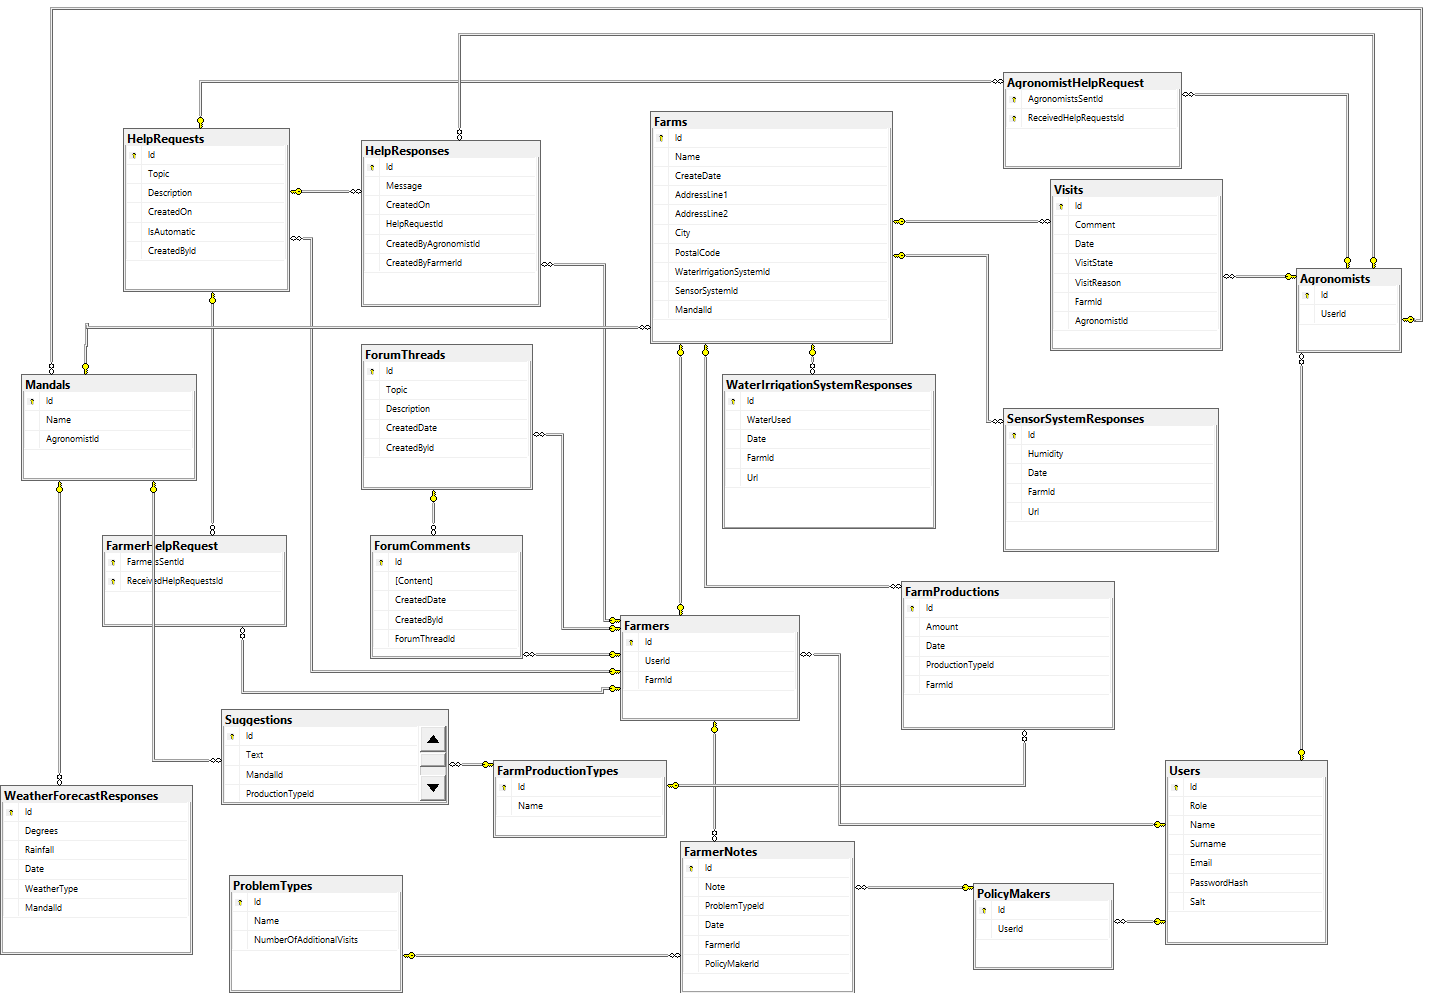
\includegraphics
    [width=\textwidth, height=0.95\textheight, keepaspectratio]
    {diagrams/database-model.png}
    \caption{Database model}
    \label{fig:db-model}
\end{figure}
